%%%%%%%%%%%%%%%%%%%%%%%%%%%%%%%%%%%%%%%%%
% Document Author: Plinio H. Vargas
% Course: CS-532, Spring 2016 at Old Dominion University
%
% Structured General Purpose Assignment
% LaTeX Template
%
% This template has been downloaded from:
% http://www.latextemplates.com
%
% Original template author:
% Ted Pavlic (http://www.tedpavlic.com)
%
% Note:
% The \lipsum[#] commands throughout this template generate dummy text
% to fill the template out. These commands should all be removed when 
% writing assignment content.
%
%%%%%%%%%%%%%%%%%%%%%%%%%%%%%%%%%%%%%%%%%
%----------------------------------------------------------------------------------------
%	PACKAGES AND OTHER DOCUMENT CONFIGURATIONS
%----------------------------------------------------------------------------------------

\documentclass{article}

\usepackage{fancyhdr} % Required for custom headers
\usepackage{lastpage} % Required to determine the last page for the footer
\usepackage{extramarks} % Required for headers and footers
\usepackage{listings}
\usepackage{graphicx} % Required to insert images
\usepackage{lipsum} % Used for inserting dummy 'Lorem ipsum' text into the template
\usepackage[bookmarks,bookmarksopen,bookmarksdepth=2]{hyperref} % for bookmarks
\usepackage{enumerate}
\usepackage{csquotes} % for quoting things
\usepackage{multirow}
\usepackage{amsmath}
\usepackage{navigator}
\usepackage{caption}
\usepackage[shortlabels]{enumitem}
\usepackage{lmodern}
\usepackage[utf8]{inputenc}
%\usepackage[table]{xcolor}% http://ctan.org/pkg/xcolo
\usepackage[dvipsnames]{xcolor}
\usepackage{longtable}
\usepackage{textcomp}
\usepackage{url}
\usepackage{import}
\usepackage{float}
\usepackage{dashrule} % for dashline
\usepackage{keystroke}

\lstdefinestyle{numbers}
{ frame=tb,
  language=python,
  aboveskip=3mm,
  belowskip=3mm,
  showstringspaces=false,
  columns=flexible,
  basicstyle={\small\ttfamily},
  numbers=left,
  numberstyle=\tiny\color{gray},
  keywordstyle=\color{blue},
  commentstyle=\color{OliveGreen},
  stringstyle=\color{purple},
  breaklines=true,
  breakatwhitespace=true,
  tabsize=3
}

\lstdefinestyle{nonumbers}
{ frame=shadowbox,
  language=python,
  aboveskip=3mm,
  belowskip=3mm,
  showstringspaces=false,
  columns=flexible,
  basicstyle={\small\ttfamily},
  numbers=none,
  numberstyle=\tiny\color{gray},
  keywordstyle=\color{blue},
  commentstyle=\color{OliveGreen},
  stringstyle=\color{purple},
  breaklines=true,
  breakatwhitespace=true,
  tabsize=3
}

\lstdefinestyle{mybox}
{
	basicstyle={\small\ttfamily},
    numbers=left,
    numberstyle=\tiny\color{gray},
    stepnumber=1,
    numbersep=5pt,
    showspaces=false, % don't show spaces by adding underscores
    showstringspaces=false, % don't underline spaces in strings
    showtabs=false, % don't show tabs with underscores
    frame=shadowbox,
    tabsize=4,
    captionpos=b,
    breaklines=true,
    breakatwhitespace=false,
  	keywordstyle=\color{blue},
	commentstyle=\color{OliveGreen},
  	stringstyle=\color{purple},    
    rulesepcolor=\color{red!20!green!20!blue!20},
    numberbychapter=false,
    stringstyle=\color{purple},
}
% Margins
\topmargin=-0.45in
\evensidemargin=0in
\oddsidemargin=0in
\textwidth=6.5in
\textheight=9.0in
\headsep=0.25in 

\linespread{1.1} % Line spacing
\newcommand*{\medtau}{\mathbin{\scalebox{1.5}{$\tau$}}}% increase size of tau
\newcommand*{\medtaub}{\mathbin{\scalebox{1.5}{$\tau_b$}}}% increase size of tau_b
\newcommand\multibrace[3]{\rdelim\}{#1}{3mm}[\pbox{#2}{#3}]}

% Set up the header and footer
\pagestyle{fancy}
\lhead{\hmwkAuthorName} % Top left header
\chead{\hmwkShortClass\ (\hmwkClassInstructor\ \hmwkClassTime): \hmwkShortTitle} % Top center header
%\rhead{\firstxmark} % Top right header
\rhead{} % Top right header
\lfoot{\lastxmark} % Bottom left footer
\cfoot{} % Bottom center footer
\rfoot{Page\ \thepage\ of\ \pageref{LastPage}} % Bottom right footer
\renewcommand\headrulewidth{0.4pt} % Size of the header rule
\renewcommand\footrulewidth{0.4pt} % Size of the footer rule

\setlength\parindent{0pt} % Removes all indentation from paragraphs

%----------------------------------------------------------------------------------------
%	DOCUMENT STRUCTURE COMMANDS
%	Skip this unless you know what you're doing
%----------------------------------------------------------------------------------------

% Header and footer for when a page split occurs within a problem environment
\newcommand{\enterProblemHeader}[1]{
\nobreak\extramarks{#1}{#1 continued on next page\ldots}\nobreak
\nobreak\extramarks{#1 (continued)}{#1 continued on next page\ldots}\nobreak
}

% Header and footer for when a page split occurs between problem environments
\newcommand{\exitProblemHeader}[1]{
\nobreak\extramarks{#1 (continued)}{#1 continued on next page\ldots}\nobreak
\nobreak\extramarks{#1}{}\nobreak
}

\setcounter{secnumdepth}{0} % Removes default section numbers
\newcounter{homeworkProblemCounter} % Creates a counter to keep track of the number of problems

\newcommand{\homeworkProblemName}{}
\newenvironment{homeworkProblem}[1][Problem \arabic{homeworkProblemCounter}]{ % Makes a new environment called homeworkProblem which takes 1 argument (custom name) but the default is "Problem #"
\stepcounter{homeworkProblemCounter} % Increase counter for number of problems
\renewcommand{\homeworkProblemName}{#1} % Assign \homeworkProblemName the name of the problem
\section{\homeworkProblemName} % Make a section in the document with the custom problem count
\enterProblemHeader{\homeworkProblemName} % Header and footer within the environment
}{
\exitProblemHeader{\homeworkProblemName} % Header and footer after the environment
}

\newcommand{\problemAnswer}[1]{ % Defines the problem answer command with the content as the only argument
\noindent\framebox[\columnwidth][c]{\begin{minipage}{0.98\columnwidth}#1\end{minipage}} % Makes the box around the problem answer and puts the content inside
}

\newcommand{\homeworkSectionName}{}
\newenvironment{homeworkSection}[1]{ % New environment for sections within homework problems, takes 1 argument - the name of the section
\renewcommand{\homeworkSectionName}{#1} % Assign \homeworkSectionName to the name of the section from the environment argument
\subsection{\homeworkSectionName} % Make a subsection with the custom name of the subsection
\enterProblemHeader{\homeworkProblemName\ [\homeworkSectionName]} % Header and footer within the environment
}{
\enterProblemHeader{\homeworkProblemName} % Header and footer after the environment
}
   
%----------------------------------------------------------------------------------------
%	NAME AND CLASS SECTION
%----------------------------------------------------------------------------------------

\newcommand{\hmwkTitle}{\\Assignment\ \#3} % Assignment title
\newcommand{\hmwkShortTitle}{Assignment 3} % Assignment title
\newcommand{\hmwkDueDate}{Thursday,\ February 18,\ 2016} % Due date
\newcommand{\hmwkClass}{CS-432/532 Introduction to Web Science} % Course/class
\newcommand{\hmwkShortClass}{CS-432/532 Web Science} % Course/class
\newcommand{\hmwkClassTime}{- Spring 2016} % Class/lecture time
\newcommand{\hmwkClassInstructor}{Dr.  Michael L. Nelson} % Teacher/lecturer
\newcommand{\hmwkAuthorName}{Plinio Vargas} % Your name
\newcommand{\hmwkAuthorEmail}{pvargas@cs.odu.edu} % Your name
%------------------------------------------------------------
% Algorithm declaration
%------------------------------------------------------------
\lstnewenvironment{algorithm}[1][] %defines the algorithm listing environment
{   
    %\refstepcounter{nalg} %increments algorithm number
    \captionsetup{labelsep=colon} %defines the caption setup for: it ises label format as the declared caption label above and makes label and caption text to be separated by a ':'
    \lstset{ %this is the stype
        frame=tB,
        numbers=left, 
        mathescape=true,
        numberstyle=\tiny,
        basicstyle={\small\ttfamily}, 
        keywordstyle=\color{blue}\bfseries\em,
        keywords={,input, output, return, 
                   datatype, function, in, 
                   if, else, for, foreach, 
                   while, write, begin, end, 
        } %add the keywords you want, or load a language as Rubens explains in his comment above.
        numbers=left,
        xleftmargin=.04\textwidth,
        #1 % this is to add specific settings to an usage of this environment (for instnce, the caption and referable label)
    }
}
{}
%----------------------------------------------------------------------------------------
%	TITLE PAGE
%----------------------------------------------------------------------------------------

\title{
\vspace{2in}
\textmd{\textbf{\hmwkClass:\ \hmwkTitle}}\\
\normalsize\vspace{0.1in}\small{Due\ on\ \hmwkDueDate}\\
\vspace{0.1in}\large{\textit{\hmwkClassInstructor\ }}
\vspace{3in}
}

\author{\textbf{\hmwkAuthorName} \\ \hmwkAuthorEmail}
\date{} % Insert date here if you want it to appear below your name

%----------------------------------------------------------------------------------------
%	EMBEDDED FILE
%----------------------------------------------------------------------------------------
%\embeddedfile{TwitterURI.py}{../TwitterURI.py}
%----------------------------------------------------------------------------------------
%	START OF DOCUMENT
%----------------------------------------------------------------------------------------
\begin{document}

\clearpage\maketitle
\thispagestyle{empty}

%----------------------------------------------------------------------------------------
%	TABLE OF CONTENTS
%----------------------------------------------------------------------------------------

%\setcounter{tocdepth}{1} % Uncomment this line if you don't want subsections listed in the ToC

\newpage
\clearpage\tableofcontents
\listoffigures
\lstlistoflistings
\listoftables

\thispagestyle{empty}
\newpage
\setcounter{page}{1}

%----------------------------------------------------------------------------------------
%	Problem 1
%----------------------------------------------------------------------------------------
\begin{homeworkProblem} % Custom section title
\vspace*{10pt} % Question
Download the 1000 URIs from assignment \#2.  \enquote{curl}, \enquote{wget}, or
\enquote{lynx} are all good candidate programs to use.  We want just the
raw HTML, not the images, stylesheets, etc.\\

from the command line:\\

\% curl http://www.cnn.com/ $>$ www.cnn.com\\

\% wget -O www.cnn.com http://www.cnn.com/\\

\% lynx -source http://www.cnn.com/ $>$ www.cnn.com\\

\enquote{www.cnn.com} is just an example output file name, keep in mind
that the shell will not like some of the characters that can occur
in URIs (e.g., "?", "\&").  You might want to hash the URIs, like:\\

\% echo -n \enquote{\url{http://www.cs.odu.edu/show_features.shtml?72}} $|$ md5\\
41d5f125d13b4bb554e6e31b6591eeb\\

(\enquote{md5sum} on some machines; note the \enquote{-n} in echo -- this removes
the trailing newline.) \\

Now use a tool to remove (most) of the HTML markup.  \enquote{lynx} will
do a fair job:\\

\% lynx -dump -force\_html www.cnn.com $>$ www.cnn.com.processed\\

Use another (better) tool if you know of one.  Keep both files 
for each URI (i.e., raw HTML and processed).\\
\vspace{10mm}

\subsection{1.1 Approach}
As suggested in the problem requirement, all URIs were hashed using \textbf{MD5} function. A python application $<\textbf{ProcessRawURI.py}>$ was developed to solve this problem.  The application makes two (2) different iterations:
\begin{enumerate}
	\item For each of the 1000 URIs, it gets a copy of the resources and saves the raw HTML content into a file: lines 29-43.
	\item Each raw file is processed to remove all HMTL markup. A system call using the \textit{lynx} command performs the HTML markup removal: 45-50. 
\end{enumerate}

\lstinputlisting[language=Python,
                 style=mybox, 
                 captionpos=t,
                 caption={ProcessRawURI.py},
                 label=listing:Raw-URI,
                 ]
{../ProcessRawURI.py}
\textbf{ProcessRawURI.py} is attached to this document.
\subsection{1.2 Solution}
All raw and processed files were stored into directory ./URI-work-files
\end{homeworkProblem}

%----------------------------------------------------------------------------------------
%	Problem 2
%----------------------------------------------------------------------------------------
\newpage
\begin{homeworkProblem}
 Choose a query term (e.g., \enquote{shadow}) that is not a stop word
(see week 5 slides) and not HTML markup from step 1 (e.g., \enquote{http})
that matches at least 10 documents (hint: use \enquote{grep} on the processed
files).  If the term is present in more than 10 documents, choose
any 10 from your list.  (If you do not end up with a list of 10
URIs, you've done something wrong).\\

As per the example in the week 5 slides, compute TFIDF values for
the term in each of the 10 documents and create a table with the
TF, IDF, and TFIDF values, as well as the corresponding URIs.  The
URIs will be ranked in decreasing order by TFIDF values.  For
example:\\

Table 1. 10 Hits for the term \enquote{shadow}, ranked by TFIDF.\\

\begin{tabular}{l l l l}
TFIDF &	TF & IDF & URI\\
\texttt{-----} & \texttt{--} & \texttt{---} & \texttt{---}\\
0.150 & 0.014 & 10.680 & http://foo.com/\\
0.044 & 0.008 & \multicolumn{1}{r}{5.510} & http://bar.com/\\
\end{tabular}
\vspace{5mm}
\\
You can use Google or Bing for the DF estimation.  To count the
number of words in the processed document (i.e., the denominator
for TF), you can use \enquote{wc}:\\

\% wc -w www.cnn.com.processed\\
   \hspace*{7mm} 2370 www.cnn.com.processed\\

It won't be completely accurate, but it will be probably be
consistently inaccurate across all files.  You can use more 
accurate methods if you'd like.  \\

Don't forget the log base 2 for IDF, and mind your significant
digits!\\

\subsection{2.1 Approach}
\begin{enumerate}[2.1.\arabic{enumi} ]
\item The query term used to select our 10 documents was \enquote{football}. A Python application \textbf{MyGrep.py} was developed to display the frequency count in which our term \enquote{football} appeared within each processed document.\\

\lstinputlisting[language=Python,
                 style=mybox, 
                 captionpos=t,
                 caption={MyGrep.py},
                 label=listing:Grep,
				 linerange={23-32},
				 firstnumber=23                 
                 ]
{../MyGrep.py}

Line 24 places into array \textbf{processed\_files} all files in our working directory with extension \enquote{processed} in its filename. The remaining of above partial code iterates through each file and display a hashed filename, word counts and the frequency of our term. Below, tail end result of executing \textbf{MyGrep.py}:\\

\begin{figure}[!h]
\caption{Querying \enquote{football} on Processed Files}\label{fig:0}
\center
\begin{tabular}{l}
1deb1fd27da216c002a66a12afa7f240.processed 60 0\\
1b5b572e91fff302c72fede1953390cc.processed 2388 0\\
df44989f4b199500ecfbee2ac4700c2f.processed 2297 0\\
e884606825dc4bfc720ed8a179dde5f4.processed 4397 0\\
cbc4499880d666e056398b219cf1c800.processed 30 0\\
a4de2b1569c7fb9fbd37139ffb6e58c3.processed 4336 2\\
7b21588f35b9bd8ce5384ab0bd319e6e.processed 269 0\\
c2e06f65fbc5bc54c039c690ce313b03.processed 1093 0\\
351b4006448877b7bfe1acb3973517f7.processed 2568 0\\
bb2d991278d0815524179e1fa5374505.processed 3400 0\\
78b1e914582e37135be1676fc75cba99.processed 2477 0\\
\colorbox{yellow}{fa3fae6bd45f974305540f33721e7f63.processed 24414 7}\\
5b4058b62dbbf161521b63bb230455b1.processed 2463 0\\
1906a0db40b28d028b74ca84dcf1f70b.processed 2845 6\\
633babe8fd450769c5ad7a8eaeabb70f.processed 1153 0\\
13cafb82717bdd4c265deab2b1a8981b.processed 2902 0\\
e3b6392348b1695a89718bdece9e6e2b.processed 2687 28\\
590a9b6bdc592cb1e564212ecb99f97d.processed 2868 0\\
0d43d0c0656d65442001287b3bc38645.processed 2524 0\\
81b74aa80d54af18eb5688ca5636fee5.processed 22880 7\\
5ab0920417dd8c6b050d05eed99ea802.processed 2488 0\\
4a0db98e86714b95fb59af5af4cc6f5b.processed 2467 0\\
d4551fea2013123d359a36af07f3c6e9.processed 2434 0\\
b1a5b6946cc705b7425769d50afb1313.processed 7166 1\\
e7b5a7e8468b7c978f975cec008bc86d.processed 1392 0\\
\\
End Time:  Tue,  Feb 16, 2016 at 05:59:22\\
Execution Time: 7.95 seconds\\
\end{tabular}
\end{figure}
\vspace{3mm}
The query resulted in 1,000 line output corresponding to: filanme processed, number of words in the file and \enquote{football} term count. For example, in Figure \ref{fig:0} the yellow highlighted output \scriptsize{fa3fae6bd45f974305540f33721e7f63.processed} \normalsize refers to a hashed URI collected from assignment 2, without any HTML markups, containing 24,414 words; 7 of them have are \enquote{football}.\\

Then, a selection of 10 line items were made from the output making sure the term count was different than 0. The selection was saved in a file: \textbf{rankedURI}.\\

\item To find the Inverse Document Frequency(\textbf{IDF}) we considered Google, using 20B for our total docs in corpus, and obtaining 1.29B for our docs with the term from the Google search \enquote{football}.\\

\begin{figure}[!h]
\caption{Google search for \enquote{football}}\label{fig:1}
\center
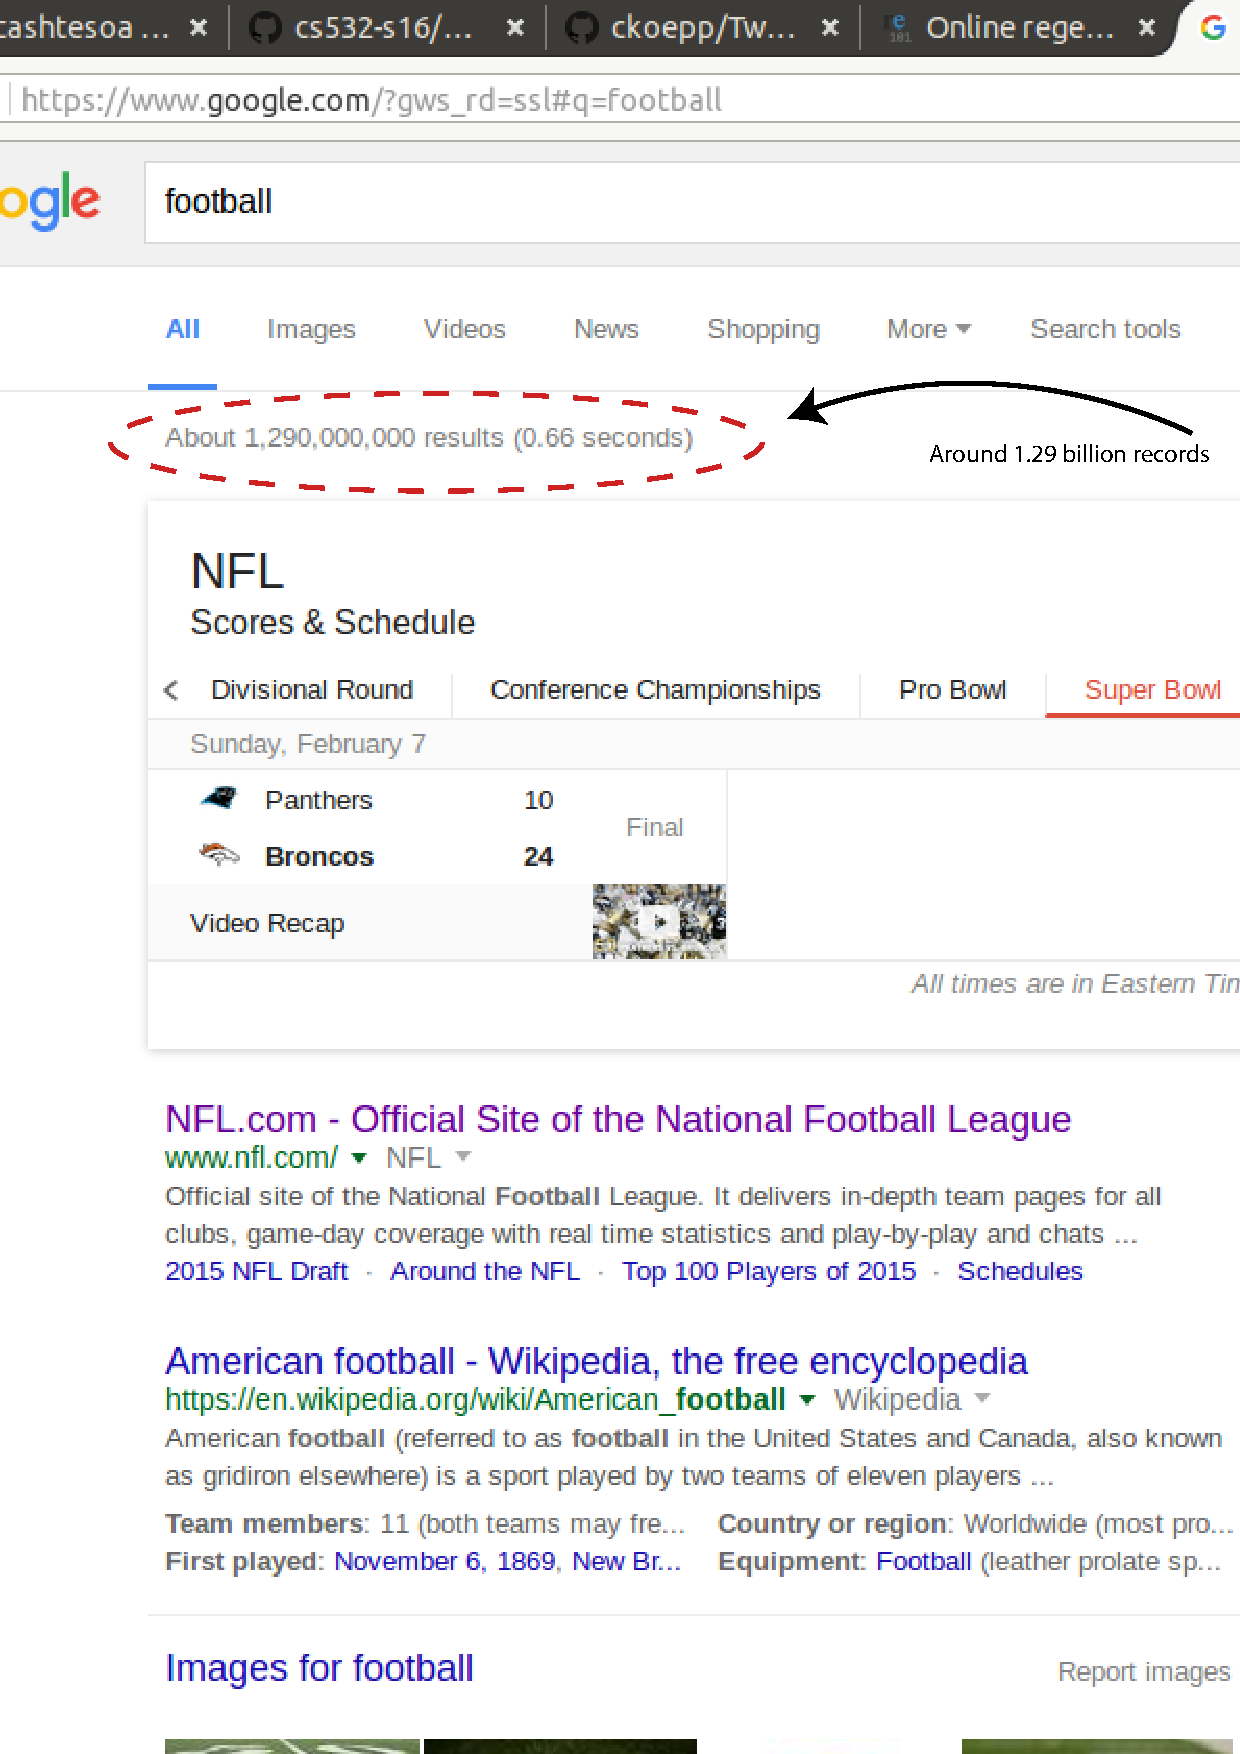
\includegraphics[scale=.5]{images/googlesearch.pdf}
\caption*{\scriptsize Result from google search of term \enquote{football} result in 1.29B records.}
\end{figure}

$total\ docus\ in\ corpus\ = $49.5B \cite{web-size} \\
$docs\ with\ term$ = 1.29B \cite{google}\\
Then,
\begin{align}
	IDF(football) &= \log_2 \Big(\frac{total\ docs\ in\ corpus}{docs\ with\ term}\Big)\\
	IDF(football) &= \log_2 \Big(\frac{49.5B}{1.29B}\Big)\\
	IDF(football) &\approx 5.262
\end{align}
%
\end{enumerate}
\newpage
\subsection{2.2 Solution}
Finally, the solution to our problem is Table \ref{tab:table1}. A Python application $<\textbf{CalculateRanking.py}>$ was developed to help calculate our 10 URIs' TFIDF score. \\
\lstinputlisting[language=Python,
                 style=mybox, 
                 captionpos=t,
                 caption={CalculateRanking.py},
                 label=listing:Grep,
				 linerange={39-59},
				 firstnumber=39                 
                 ]
{../CalculateRanking.py}
\vspace{5mm}
Lines 39-41 places our 1000 collected URIs into a hashed dictionary. Lines 43-53 iterates through our 10 selected processed files located in \textbf{rankedURI}, getting word count and TF for each file. Line 53 places into an array the calculated values for each URI: TF, IDF, TFIDF. \textbf{Note}: IDF was previously calculated. Since we have only one term, IDF is a constant.
%----------------------------------------------------------------------------------------
%	Table 1
%--------------------------------------------------------------------------------------
\import{./}{table1.tex}

\end{homeworkProblem}

%----------------------------------------------------------------------------------------
%	Problem 3
%----------------------------------------------------------------------------------------
\newpage
\begin{homeworkProblem}
Now rank the same 10 URIs from question \#2, but this time 
by their PageRank.  Use any of the free PR estimaters on the web,
such as:\\

http://www.prchecker.info/check\_page\_rank.php\\
http://www.seocentro.com/tools/search-engines/pagerank.html\\
http://www.checkpagerank.net/\\

If you use these tools, you'll have to do so by hand (they have
anti-bot captchas), but there is only 10.  Normalize the values
they give you to be from 0 to 1.0.  Use the same tool on all 10
(again, consistency is more important than accuracy).\\

Create a table similar to Table 1:\\

Table 2.  10 hits for the term \enquote{shadow}, ranked by PageRank.\\

\begin{tabular}{l l}
PageRank & URI\\
\texttt{--------} & \texttt{---}\\
0.9 & http://bar.com/\\
0.5	& http://foo.com/\\
\end{tabular}
\vspace*{5mm}
\\
Briefly compare and contrast the rankings produced in questions 2
and 3.

\newpage
\subsection{3.1 Approach}
Table \ref{tab:table2} was completed utilizing \url{http://www.seocentro.com/tools/search-engines/pagerank.html} free PR estimate:\\

\subsection{3.2 Solution}
%----------------------------------------------------------------------------------------
%	Table 2
%--------------------------------------------------------------------------------------
\import{./}{table2.tex}

\newpage
\subsection{3.3 Solutions 2 and 3 Comparison}
\begin{figure}[!h]
\caption{TFIDF Ranking vs PageRanking Comparison}\label{fig:3}
\center
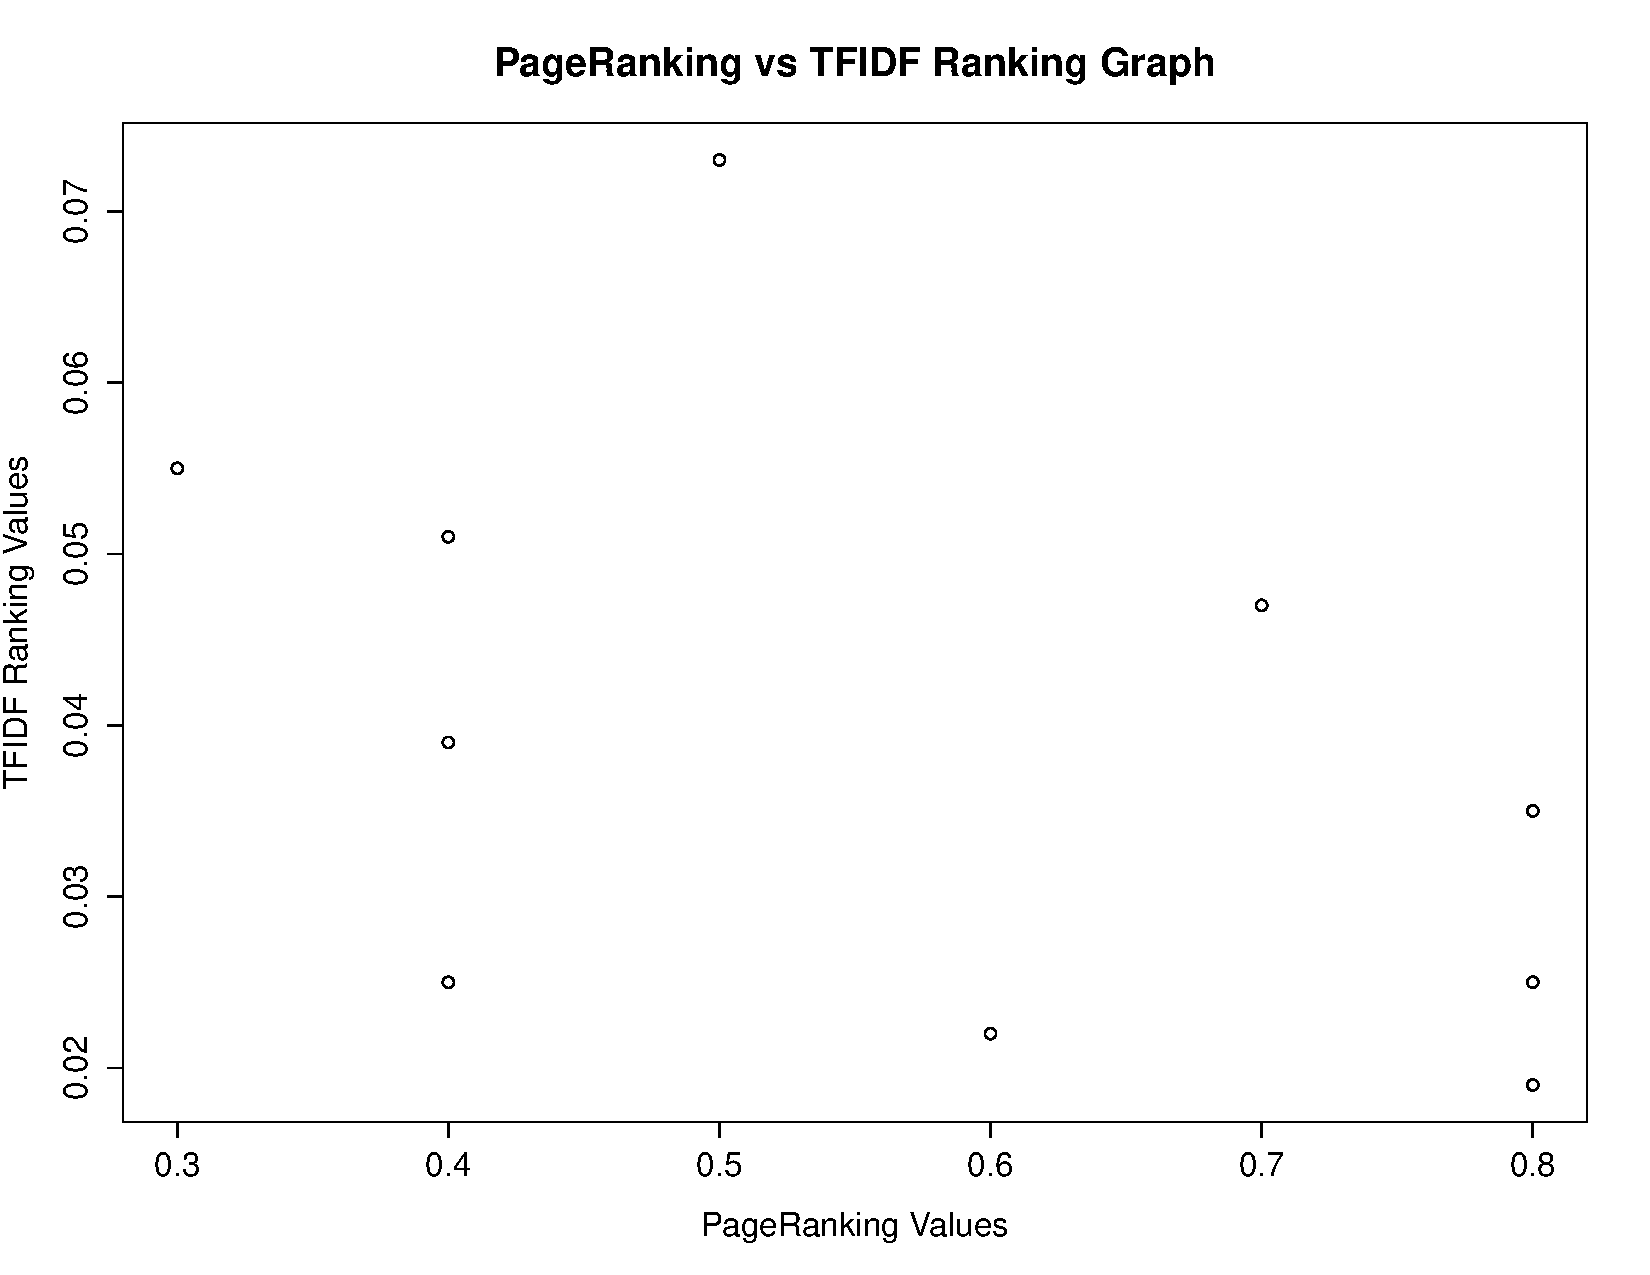
\includegraphics[scale=.5]{images/page-tfidf.pdf}
\caption*{\scriptsize Plots are all over the graph. There is not a plot grouping or a pattern identifying a relationship between PageRanking and TFIDF Ranking. This is expected since TFIDF Ranking is based on TF and it is related to the URI. The information for PageRanking is not taking in consideration our term \enquote{football} and it is not ranking the URI, but rather its root domain.}
\end{figure}
\end{homeworkProblem}

%----------------------------------------------------------------------------------------
%	Problem 4 Extra Credit
%----------------------------------------------------------------------------------------
\newpage
\begin{homeworkProblem}[Problem 4 Extra Credit]
Compute the Kendall $\medtaub$ score for both lists (use \enquote{b} because
there will likely be tie values in the rankings).  Report both the
$\medtau$ value and the \enquote{p} value.\\

\subsection{4.1 Manual Calculation}
See: \\
\url{http://stackoverflow.com/questions/2557863/measures-of-association-in-r-kendalls-tau-b-and-tau-c}\\
\url{http://en.wikipedia.org/wiki/Kendall_tau_rank_correlation_coefficient#Tau-b}\\
\url{http://en.wikipedia.org/wiki/Correlation_and_dependence}\\

According to \cite{tau-b}
\begin{align}
	\tau_B &= \frac{n_c - n_d}{\sqrt{(n_0 - n1)(n_0 - n_2)}}\\
\end{align}
where
\begin{align}
	n_0 &= n(n - 1)/2\\
	n_1 &= \sum\limits_i t_i(t_i - 1)/2\\
	n_2 &= \sum\limits_j u_j(u_i - 1)/2
\end{align}
$n_c =$ Number of concordant pairs\\
$n_d =$ Number of discordant pairs\\
$t_i =$ Number of tied values in the $i^{th}$ group of ties for the first quantity\\
$u_j =$ Number of tied values in the $j^{th}$ group of ties for the second quantity\\

%----------------------------------------------------------------------------------------
%	Table 3
%--------------------------------------------------------------------------------------
\import{./}{table3.tex}
\vspace{5mm}
$n_0 = n(n - 1)/2 = 10(9)/2 = 5(9) = 45$\\
$n_1 = \sum\limits_i t_i(t_i - 1)/2 = 2$\hspace*{15mm}
$n_2 = \sum\limits_j u_j(u_i - 1)/2 = 0$\\
$$\tau_B = \frac{n_c - n_d}{\sqrt{(n_0 - n1)(n_0 - n_2)}} = \frac{16 - 29}{\sqrt{(45 - 2)(45 - 0)}} = -\frac{13}{\sqrt{1935}} \approx -0.296$$

\subsection{4.2 R\_Studio Results}
The data comparison between RankPage and TFIDF values is contained in file \textbf{$<$page-tfidf-data$>$}. Uploading the data into \enquote{R} yields the following result:\\
\begin{lstlisting}[style=nonumbers]
> Kendall::Kendall(y,x)
tau = -0.435, 2-sided pvalue =0.11572
\end{lstlisting}

\subsection{4.3 Conclusion}
According to \cite{tau-b}:
\begin{itemize}
	\item If the agreement between the two rankings is perfect (i.e., the two rankings are the same) the coefficient has value 1.
	\item If the disagreement between the two rankings is perfect (i.e., one ranking is the reverse of the other) the coefficient has value -1.
	\item If X and Y are independent, then we would expect the coefficient to be approximately zero.
\end{itemize}

Then, by the predicates above, we can conclude PageRanking and TFIDF Ranking variables are independent since the coefficient results are not close to 1 or -1, neither in the manual calculation (4.1), nor the \enquote{R} calculation (4.2). Additionally, Figure \ref{fig:3} demonstrates in the graph how scattered the plots are between their values.
\end{homeworkProblem}

%----------------------------------------------------------------------------------------
%	Bibliography
%----------------------------------------------------------------------------------------
\newpage
\begin{thebibliography}{9}
%\bibitem{Lutz} 
%Lutz, Mark (2013). List and Dictionaries. \textit{Learning Python} (5th ed.). (pp. %262-263). Sebastopol, CA: O'Reilly Media.
%
\bibitem{tau-b}
Graph structure in the web. (n.d.) Retrieved February 15, 2016, from \url{https://en.wikipedia.org/wiki/Kendall_rank_correlation_coefficient#Tau-b}

\bibitem{web-size}
Daily Estimate Size of the World Wide Web. (n.d.) Retrieve February 17, 2015, from \url{http://www.worldwidewebsize.com/}

\bibitem{google}
Football Google Search. (n.d.) Retrieve February 17, 2015, from \url{http://www.google.com/?gws_rd=ssl#q=football/}
\end{thebibliography}
\end{document}
